%
% Draft  document voidlumina.tex
%
 
\documentclass{article}  % Latex2e
\usepackage{graphicx,lscape,subfigure}
 

\title{My experiences with setting up the Lumina desktop in Void linux}
\author{Neville Jackson}
\date{18 May 2022} 

\begin{document} 

\maketitle      

\section{Introduction} 
The {\em Lumina Desktop} is an OS-independent desktop environment which can be ported to BSD, Linux or OS-X. It was developed in the BSD community, and is part of the TrueOS and Project Trident distributions. Both TrueOS and Trident are now discontinued, but Lumina is still active. 

There is a lumina website~\cite{lumi:22} and there are ports (BSD) or packages (Linux) available for all the BSD's, and for antiX, Arch, Debian, Fedora, Gentoo, Manjaro, NixoS, PCLinuxOS, and Void Linux. Lumina has  BSD licence.

I wanted to try Lumina in Void Linux, partly because of my BSD background, and partly because I thought the collapsed Project Trident was a loss. There is a FOSS article~\cite{foss:21} on Project Trident. 

What I am doing here is not an attempt to resurrect Trident. Trident used the ZFS filesystem. I am staying with ext4. I just want to see if it is possible to setup a reasonable working environment using Lumina Desktop in Void Linux. 

Some of the major features of Lumina are
\begin{itemize}
\item the lumina package comes with a minimum of applications. You have to add your choice of apps.
\item lumina uses qt5 (but not QML), and X11. It has not gone to Wayland yet.
\item lumina is built on top of the Fluxbox window manager
\item lumina has all the features of a modern desktop - desktop widgets like KDE, plugins (embedded objects like KDE plasmids), app menu, app icons, highly configurable. 
\end{itemize}

The only way to really test Lumina is to use it... daily for normal work.  This document reports on setting up Lumina and on usage.

\section{Install Void Linux }
\label{sec:install}
The comptuter used  was a desktop with the following hardware 
\begin{verbatim}
Machine:
  Type: Desktop Mobo: ASUSTeK model: P9X79 DELUXE v: Rev 1.xx 
  serial: <filter> UEFI: American Megatrends v: 1203 date: 05/24/2012 
CPU:
  Info: 6-Core model: Intel Core i7-3930K bits: 64 type: MT MCP 
  arch: Sandy Bridge family: 6 model-id: 2D (45) stepping: 7 
  .............
\end{verbatim}
There should be no performance issues, the computer is about 10 years old but has ample cpu power and 64Gb of ram.

The approach taken was to  do a minimal install of Void then attempt to add the lumina desktop.

The Void linux download page is at
\begin{verbatim}
https://voidlinux.org/download/
\end{verbatim}
Void downloads are available either with the graphical Xfce desktop environment, or as a plain command line {\em base} image. For this job I chose the base .iso file, with glibc libraries, as I did not want to have to remove Xfce.

The void-live-x86\_64-20210930.iso file (542Mb) was downloaded and installed to a 186Gb pre-prepared partition with an ext4 filesystem. There were existing swap spaces. The /home directory was left on the root filesystem. An existing grub2 was used to boot.
\subsection{Installation procedure}
{\bf Do a backup first}
Make a bootable live Void linux device (DVD or USB drive) from the downloaded .iso file.
The Void installer is a non-graphical program, which you simply run after booting the live system. On booting you are told there is a root user with the password of voidlinux, and a user called anon with the same password. So to start the installer do
\begin{verbatim}
# void-installer
\end{verbatim}
and it will march you thru a menu of steps as follows
\begin{verbatim}
keyboard:
network:
source: is it local install from media or over network
hostname:
locale:
timezone:
root passwd:
user account:
bootloader:
partition:
filesystems: choose partition(s), setup mount point(s):
install: copies Void to the '/' partition
\end{verbatim}
I bypassed the bootloader: and partitions: sections as I already had a bootloader and a prepared partition for the root filesystem. 

{\bf Warning: The one trap which I have found is that when you get to the filesystems: section, if you have more than one disk in your system, the void-installer seems to label them in random order - ie which disk is /sda and which is /sdb today , may not be the same next time you use the installer, and may not be the same as other Linux versions on your computer use. So if you are looking to put the Void rootfilesystem on what you know as /sda1, for example, it is very easy to make a mistake and end up overwriting /sdb1. Be very careful!  Use the filesystem sizes to check that the installer is going to write on the coreect partition! }

After the installation completes, you will need to boot into the version of Linux that controls grub, in my case Debian 11, and redo the grub configuration as follows
\begin{verbatim}
update-grub
\end{verbatim}
It should find all your operating systems, including the new Void install. 

If it does not find everything check that {\em os-prober} is enabled. Go to {\em /etc/default} and edit the file {\em grub} adding the line
\begin{verbatim}
GRUB_DISABLE_OS_PROBER=false
\end{verbatim}
Then update-grub should find everything.

We can now power off, remove the Void install medium, boot, and choose the new Void install from the gub menu.


\section{Setup Void linux}
At first boot, you get a login prompt on a terminal screen. No window system, no graphical login screen. So login as root and do a full system update using the {\em xbps} package manager. Void has its own package manager - it does not use either {\em apt} or {\em rpm}. Xbpm stands for X binary package manager - it is unique to Void, but it is efficient and easy to learn. 

To do a full system update we do
\begin{verbatim}
xbps-install -Su
\end{verbatim}
Mine downloaded 269Mb, so be prepared for a short wait. 
What that achieves is to bring all installed packages plus Linux up to date. Void is a managed rolling release distro. One needs to do a system update at least once a month. You will never have to do a reinstall of a major release, there are none. The monthly updates keep Void at the latest release forever.

We are now ready to try and install a desktop

\section{Install lumina desktop}
A search for the lumina desktop using the {\em xbps} package commands leads to
\begin{verbatim}
# xbps-query -Rs lumina
[-] lumina-1.6.0_2            Lumina Desktop Environment
[-] lumina-calculator-1.6.0_1 Scientific calculator from the Lumina desktop
[-] lumina-pdf-1.6.0_1        PDF reader and presentation utility from the Lu...
[-] lumina-32bit-1.6.0_2      Lumina Desktop Environment (32bit)
\end{verbatim}
 So only 3 packages ( ignoring the 32-bit one). The {\em -Rs} option on {\em xbps-query} tells it to search the repository and installed packages. 

That is version 1.6.0 of lumina; the lumina website 
\begin{verbatim}
https://lumina-desktop.org/
\end{verbatim}
says the latest release of lumina is 1.6.2?  The Void repository is normally more up to date than that?

 Go ahead and install lumina
\begin{verbatim}
# xbps-install lumina
160 packages will be downloaded:

160 packages will be installed:
  fluxbox-1.3.7_3 numlockx-1.2_5 xbacklight-1.2.3_1 acpi-1.7_4 
  ................
  qt5-gui-5.15.3+20220222_1 qt5-widgets-5.15.3+20220222_1 
  ..............
  qt5-multimedia-5.15.3+20220222_1 lumina-1.6.0_2

Size to download:               121MB
Size required on disk:         405MB
Space available on disk:       270GB

Do you want to continue? [Y/n] 
\end{verbatim}
So say yes and let it install . Lumina is built on top of fluxbox, and requires qt5 and a few other things, but it is really quite a minimal size. Compare 121Mb with KDE's 447Mb.

Repeat the {\em xbps-install} for the other two packages associated with lumin
\begin{verbatim}
xbps-install lumina-calculator
xbps-install lumina-pdf
\end{verbatim}
This downloaded another 5.2Mb. They are small addon packages

I need to reboot now and see what we have got. How to reboot from the command line? The old fashioned way
\begin{verbatim}
sync
sync
halt
\end{verbatim}
That will power you right off instantly. Why two sync's? Superstition. You really need to do sync before halt, so doing it twice protects you against typos. If you ar queasy about halt, use shutdown.

Then boot the new Void again, and what do we get? Same as before - a terminal login. That is because we have only installed the DTE - ie the Window Manager plus extras. There is no Display Manager - commonly called login screen. So the lumina install did not drag in a display manager? Never mind, we can install it separately.

For now, we will just login again at the terminal, and try starting lumina. The start script for X11 is normally {\em /usr/bin/startx} but in the case of lumina it is {\em /usr/bin/start-lumina-desktop}. There is also a start script for fluxbox {\em /usr/bin/startfluxbox}. So type
\begin{verbatim}
start-lumina-desktop
\end{verbatim}
and we get a lumina desktop screen. It looks like Figure~\ref{fig:lumina1}
%\documentclass{article}
%\usepackage{graphicx,subfigure}
%\begin{document}

\begin{figure}[!h]
  \centering
   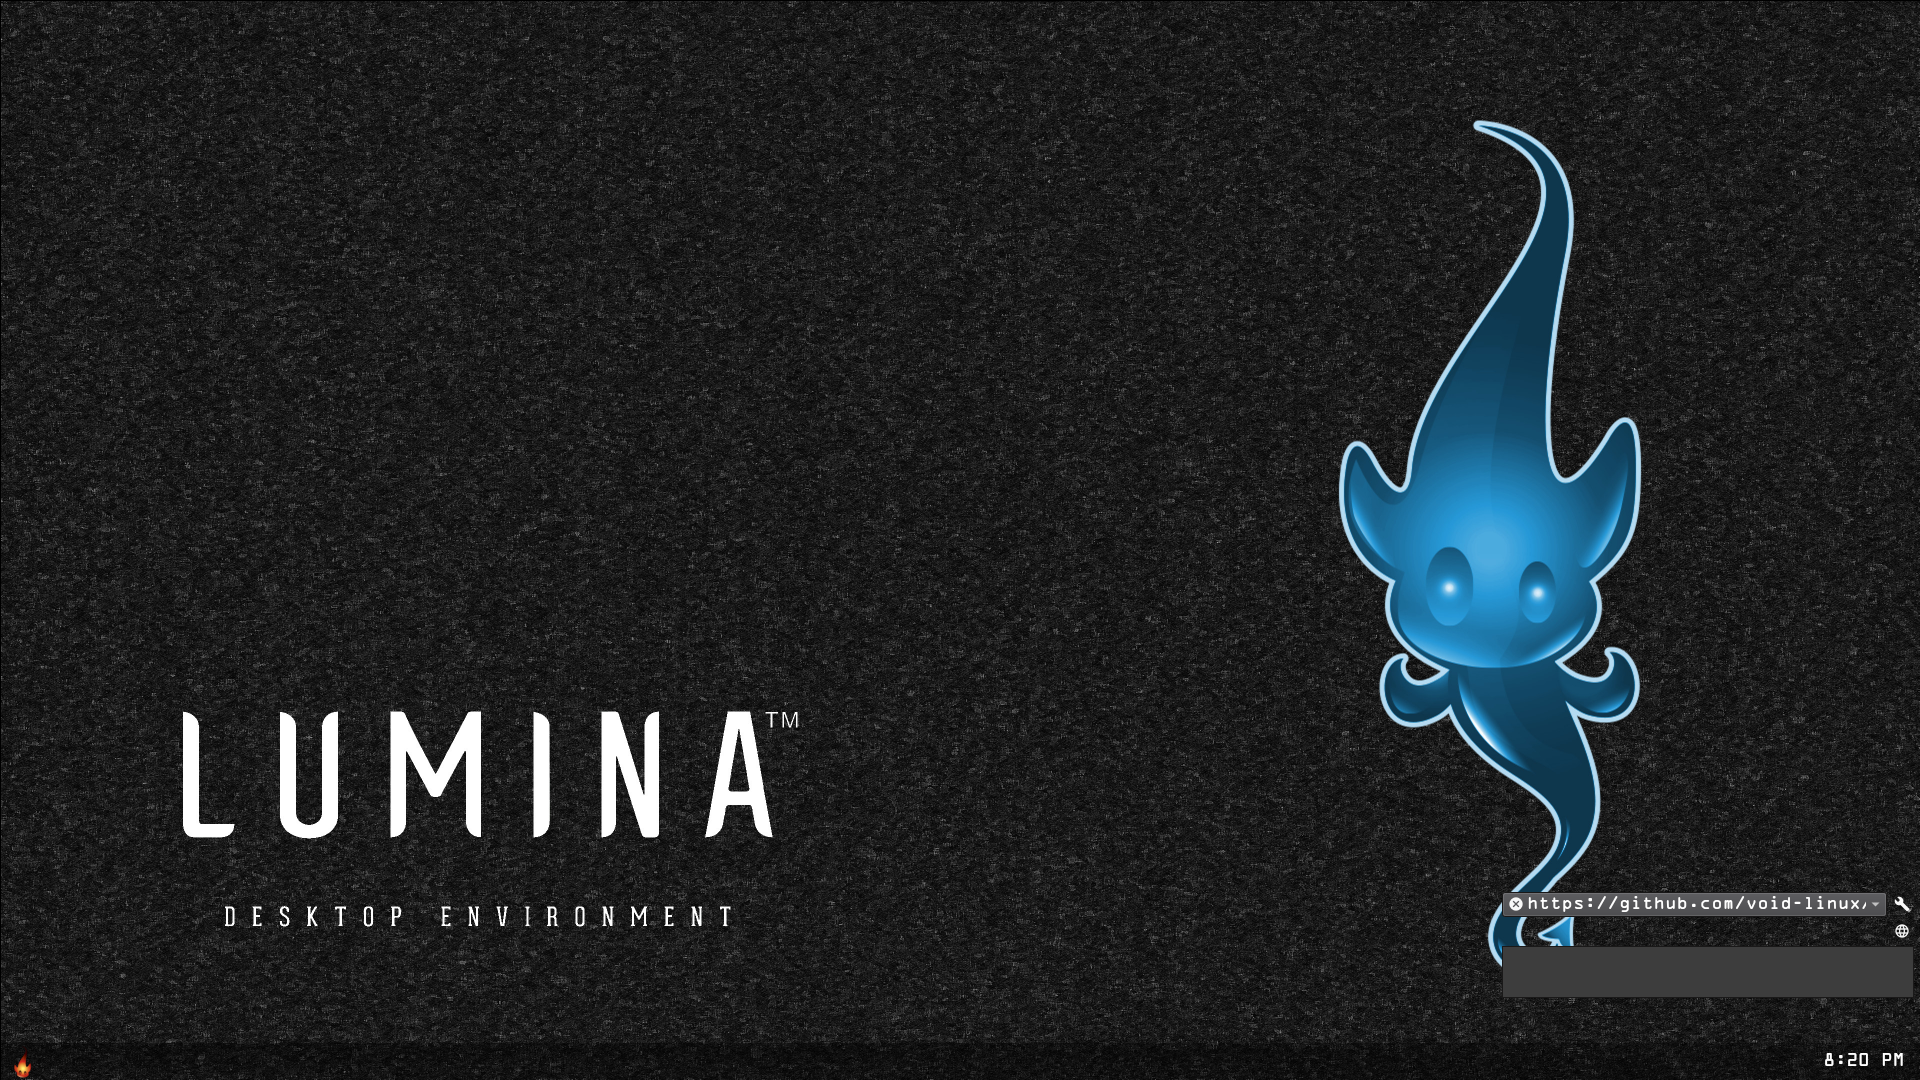
\includegraphics[totalheight=3in,width=1.0\textwidth]{lumina1.png}
  \caption{Screenshot of initial Lumina screen with default configuration and no additional installs}
  \label{fig:lumina1}
\end{figure}

%\end{document}


It is quite minimal. There is a 'flame' icon in the bottom panel at the left - this brings a menu (Figure~\ref{fig:menu12}a) offering Files, Applications, Preferences, and Leave Options. The Applications choice expands into a menu of included software (Figure~\ref{fig:menu12}b) among which you will find the Lumina Screenshot App used to obtain these shots.   
%\documentclass{article}
%\usepackage{graphicx,subfigure}
%\usepackage{caption,rotating}
%\begin{document}

\begin{figure}[p]
\centering
 \subfigure[First menu]{
    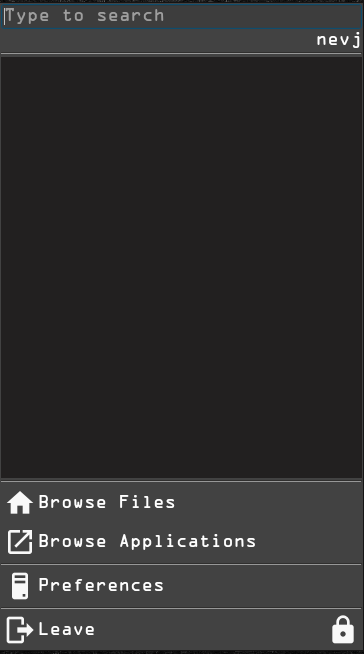
\includegraphics[scale=0.50]{menu1.png}
  }
 \subfigure[Second menu within Applications]{
    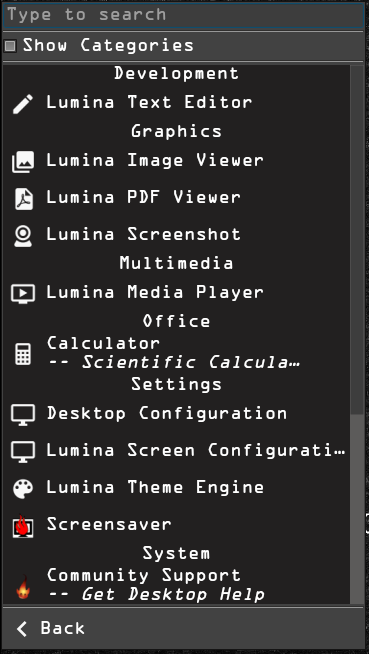
\includegraphics[scale=0.50]{menu2.png}
  }
  \caption{Screenshot of menu obtained from click on 'flame' icon at left of bottom panel of Lumina desktop}
\vfill
  \label{fig:menu12}
\end{figure}

%\end{document}



There is a time widget in the bottom panel at the right, and there is a floating widget ( like a plasmoid in KDE) on the lower right displaying a web address. That floating widget is actually for an RSS feed. Clicking on the tool icon beside it changes it to a display of recent commits to void-packages:master, as shown in Figure~\ref{fig:menu34}a.

 Right click on the screen background displays a second menu, (Figure~\ref{fig:menu34}b),  in the samne manner as most desktops, offering the same same choices again , plus Terminal ( it means Editor not Xterm) and Desktop Actions.
%\documentclass{article}
%\usepackage{graphicx,subfigure}
%\usepackage{caption,rotating}
%\begin{document}

\begin{figure}[p]
\centering
 \subfigure[Embedded RSS feed widget]{
    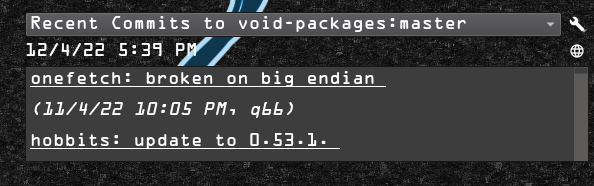
\includegraphics[scale=0.50]{widget.png}
  }
 \subfigure[Background right click menu]{
    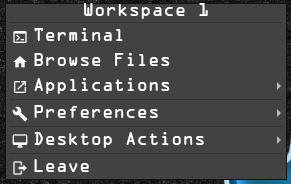
\includegraphics[scale=0.50]{menu3.png}
  }
  \caption{Screenshots of embedded RSS feed widget and background right click menu}
\vfill
  \label{fig:menu34}
\end{figure}

%\end{document}



 Any application can be displayed in a floating widget. As an example I have added {\em System Monitor} to the list of what it calls Embedded Utilities in the Desktop Settings Menu. This brings up a second floating widget. The result is shown in Figure~\ref{fig:embed}
%\documentclass{article}
%\usepackage{graphicx,subfigure}
%\begin{document}

\begin{figure}[!h]
  \centering
   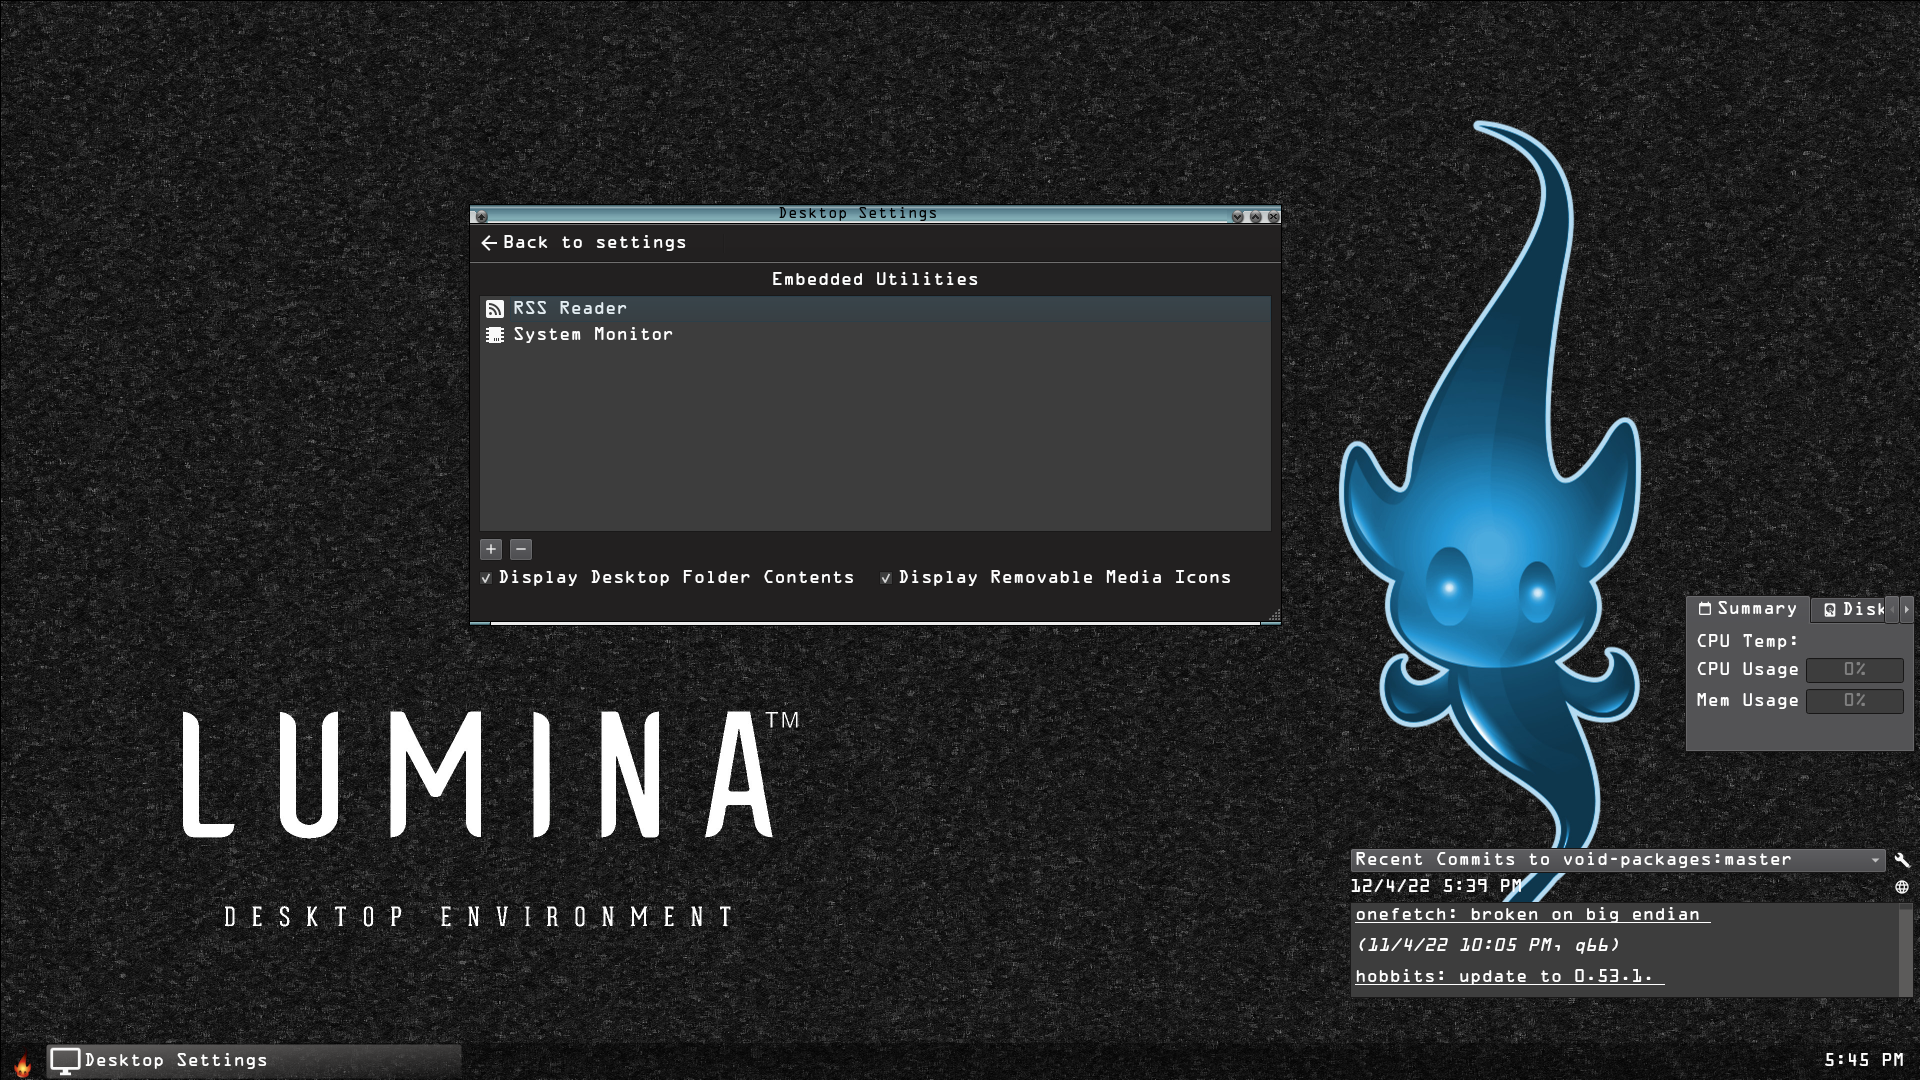
\includegraphics[totalheight=3in,width=1.0\textwidth]{embed.png}
  \caption{Screenshot showing a System Monitor background widget in addition to the default RSS Feed widget. The Desktop Settings menu used to add the widget is also displayed}
  \label{fig:embed}
\end{figure}

%\end{document}




Overall not very different from most desktops, and quite innovative in that it has floating background widgets, which are like KDE plasmoid widgets. It is stated that one can embed any Application as a background widget. That is a bit different from KDE where plasmoids are defined separately from Applications. It may have advantages. Further investigation is needed. 

 There is one glaring omission. No X-terminal anywhere? I cannot get a command line or a shell. It turns out that {\em xterm} has not been installed either by the Void base system or along with the Lumina package.  So I cant do anything. No choice but to exit and go back to the terminal prompt. 


\clearpage
\subsection{Add an XTerm}
Boot and login from the terminal prompt again.
Look in the Void repository for terminals
\begin{verbatim}
$ xbps-query -Rs xterm
[-] lxterminal-0.4.0_1           LXDE Terminal emulator
[-] roxterm-3.12.1_1             Highly configurable terminal emulator
[-] xterm-372_1                  X Terminal Emulator
[-] xtermcontrol-3.8_1           Enables dynamic control of xterm properties
\end{verbatim}
Not a lot of choice. We shall stay with the original X11 xterm for now
\begin{verbatim}
[nevj@trinity ~]$ su
Password: 
# xbps-install xterm

Name        Action    Version           New version            Download size
libutempter install   -                 1.2.1_1                5597B 
xterm       install   -                 372_1                  432KB 

Size to download:              438KB
Size required on disk:        1294KB
Space available on disk:       270GB

Do you want to continue? [Y/n] y

[*] Downloading packages
libutempter-1.2.1_1.x86_64.xbps.sig: 512B [avg rate: 13MB/s]
libutempter-1.2.1_1.x86_64.xbps: 5597B [avg rate: 67MB/s]
libutempter-1.2.1_1: verifying RSA signature...
xterm-372_1.x86_64.xbps.sig: 512B [avg rate: 10MB/s]
xterm-372_1.x86_64.xbps: 432KB [avg rate: 2718B/s]
xterm-372_1: verifying RSA signature...

[*] Collecting package files
libutempter-1.2.1_1: collecting files...
xterm-372_1: collecting files...

[*] Unpacking packages
libutempter-1.2.1_1: unpacking ...
xterm-372_1: unpacking ...

[*] Configuring unpacked packages
libutempter-1.2.1_1: configuring ...
libutempter-1.2.1_1: installed successfully.
xterm-372_1: configuring ...
Updating MIME database...
xterm-372_1: installed successfully.

2 downloaded, 2 installed, 0 updated, 2 configured, 0 removed.
# 
\end{verbatim}
It is quite small ... only 438Kb download. 

Now an XTerm and a UXTerm entry appear in the Browse Applications menu. So newly added packages get added automatically to the Apps Menu. 

Start an XTerm. It comes up in a tiny window about half normal size, with black text on a white background and no scrollbar. Absolutely minimal, but that can be configured. It is done in a file called {\em .Xresources} in the users home directory. Xresources is not an easy thing to compose from scratch, but we can copy one from elsewhere
\begin{verbatim}
xterm*faceName: Hack
xterm*faceSize: 10

xterm*loginshell: true
xterm*saveLines: 4096

!double-click to select whole URLs
xterm*charClass: 33:48,36-47:48,58-59:48,61:48,63-64:48,95:48,126:48

!DOS-box colours
xterm*foreground: rgb:a8/a8/a8
xterm*background: rgb:00/00/00
xterm*color0: rgb:00/00/00
xterm*color1: rgb:a8/00/00
xterm*color2: rgb:00/a8/00
xterm*color3: rgb:a8/54/00
xterm*color4: rgb:00/00/a8
xterm*color5: rgb:a8/00/a8
xterm*color6: rgb:00/a8/a8
xterm*color7: rgb:a8/a8/a8
xterm*color8: rgb:54/54/54
xterm*color9: rgb:fc/54/54
xterm*color10: rgb:54/fc/54
xterm*color11: rgb:fc/fc/54
xterm*color12: rgb:54/54/fc
xterm*color13: rgb:fc/54/fc
xterm*color14: rgb:54/fc/fc
xterm*color15: rgb:fc/fc/fc

!right hand side scrollbar
xterm*ScrollBar: true
xterm*rightScrollBar: true

!stop output to terminal from jumping down to bottom of scroll again
xterm*scrollTtyOutput: false
xterm*metaSendsEscape: true
\end{verbatim}
So, install this file in my home directory, start another XTerm, and what happens ... nothing. Same as before. 

Read a bit. Discover that I have to tell it to merge in the new .Xresources file with {\em xrdb} 
\begin{verbatim}
nevj@trinity ~]$ which xrdb
which: no xrdb in (/usr/local/bin:/bin:/usr/bin:/usr/local/sbin:/usr/sbin:/sbin)
\end{verbatim}
OK, so we have to install {\em xrdb}
\begin{verbatim}
[nevj@trinity ~]$ su
Password: 
# xbps-install xrdb

Name    Action    Version           New version            Download size
libmcpp install   -                 2.7.2_8                63KB 
mcpp    install   -                 2.7.2_8                165KB 
xrdb    install   -                 1.2.1_1                20KB 

Size to download:              250KB
Size required on disk:         976KB
Space available on disk:       270GB

Do you want to continue? [Y/n] y
........
\end{verbatim}
Then we can do 
\begin{verbatim}
xrdb -merge ~/.Xresources
\end{verbatim}
Now, the current XTerm stays the same, but when I start a new XTerm it comes up twice the size ( ie normal) with white text on a black backgoound, and a scrollbar on the right.  That is reasonable.

What happens on a reboot? Try it and see. Failure, the original tiny XTerm returns. So the {\em xrdb} command is temporary, the new .Xresources file is not being used after reboot?

I discover that in {\em /etc/X11/xinit} there is a file {\em xinitrc} which contains
\begin{verbatim}
#!/bin/sh

userresources=$HOME/.Xresources
usermodmap=$HOME/.Xmodmap
sysresources=/etc/X11/xinit/.Xresources
sysmodmap=/etc/X11/xinit/.Xmodmap

# merge in defaults and keymaps

if [ -f $sysresources ]; then


    xrdb -merge $sysresources

fi

if [ -f $sysmodmap ]; then
    xmodmap $sysmodmap
fi

if [ -f "$userresources" ]; then

    xrdb -merge "$userresources"

fi

if [ -f "$usermodmap" ]; then
    xmodmap "$usermodmap"
fi

# start some nice programs

if [ -d /etc/X11/xinit/xinitrc.d ] ; then
 for f in /etc/X11/xinit/xinitrc.d/?*.sh ; do
  [ -x "$f" ] && . "$f"
 done
 unset f
fi

twm &
xclock -geometry 50x50-1+1 &
xterm -geometry 80x50+494+51 &
xterm -geometry 80x20+494-0 &
exec xterm -geometry 80x66+0+0 -name login
\end{verbatim}

So if it is using this {\em xinitrc} script it should be looking at {\em \$HOME/.Xresources} but it is not. I decide to try putting the .Xresources file here ( in /etc/X11/xinit) , because there is no .Xresources file present in this directory, yet the xinitrc script looks for one. This does not fix the issue. 

I try putting 
\begin{verbatim}
xrdb -merge /etc/X11/xinit/.Xresources 
\end{verbatim}
in {\em /etc/rc.local}. This should execute it every time Void starts up. Still no success. 

Then I think, maybe Lumina does not use the .Xresources file or the {\em xinitrc} script -- maybe it uses old fashioned .Xdefaults file. So I copy .Xresources to .Xdefaults in my home directory. Reboot, and it works. 
The changes to XTerm are permanent - ie they survive a reboot. Done! We have a usable terminal.

I fiddle with the Window Themes to try and get the best xterm layout. Change from {\em Arch} to {\em Outcomes} seems appropriate, but there are no colours? Discover that the RGB color database for X11 is not installed
\begin{verbatim}
xbps-query -Rs rgb
[-] ckb-next-0.4.4_2    Corsair RGB Driver for Linux
[-] ite8291r3-ctl-0.3_1 Userspace driver for the ITE 8291 RGB keyboard backlight...
[-] openrgb-0.7_1       Open source RGB lighting control
[-] rgb-1.0.6_2         RGB color database for X11
\end{verbatim}
so install it
\begin{verbatim}
# xbps-install rgb

Name Action    Version           New version            Download size
rgb  install   -                 1.0.6_2                8628B 

Size to download:              9140B
Size required on disk:          32KB
Space available on disk:       270GB

Do you want to continue? [Y/n] 
\end{verbatim}
Then reboot, and all the windows, including xterm, have a bit of color in the frame.

Just for fun, we might try embedding an xterm app in the screen background. So add Xterm to the list of Embedded Utilities in the Desktop Settings Menu. I dont get a whole embedded XTerm, what I get is an XTerm icon. When I double click the icon I get an XTerm. That makes sense, and it is convenient to have an XTerm icon, so leave it there. 

We end with a screenshot showing  two XTerm windows and the Xterm icon (Figure~\ref{fig:xterm})
%\documentclass{article}
%\usepackage{graphicx,subfigure}
%\begin{document}

\begin{figure}[!h]
  \centering
   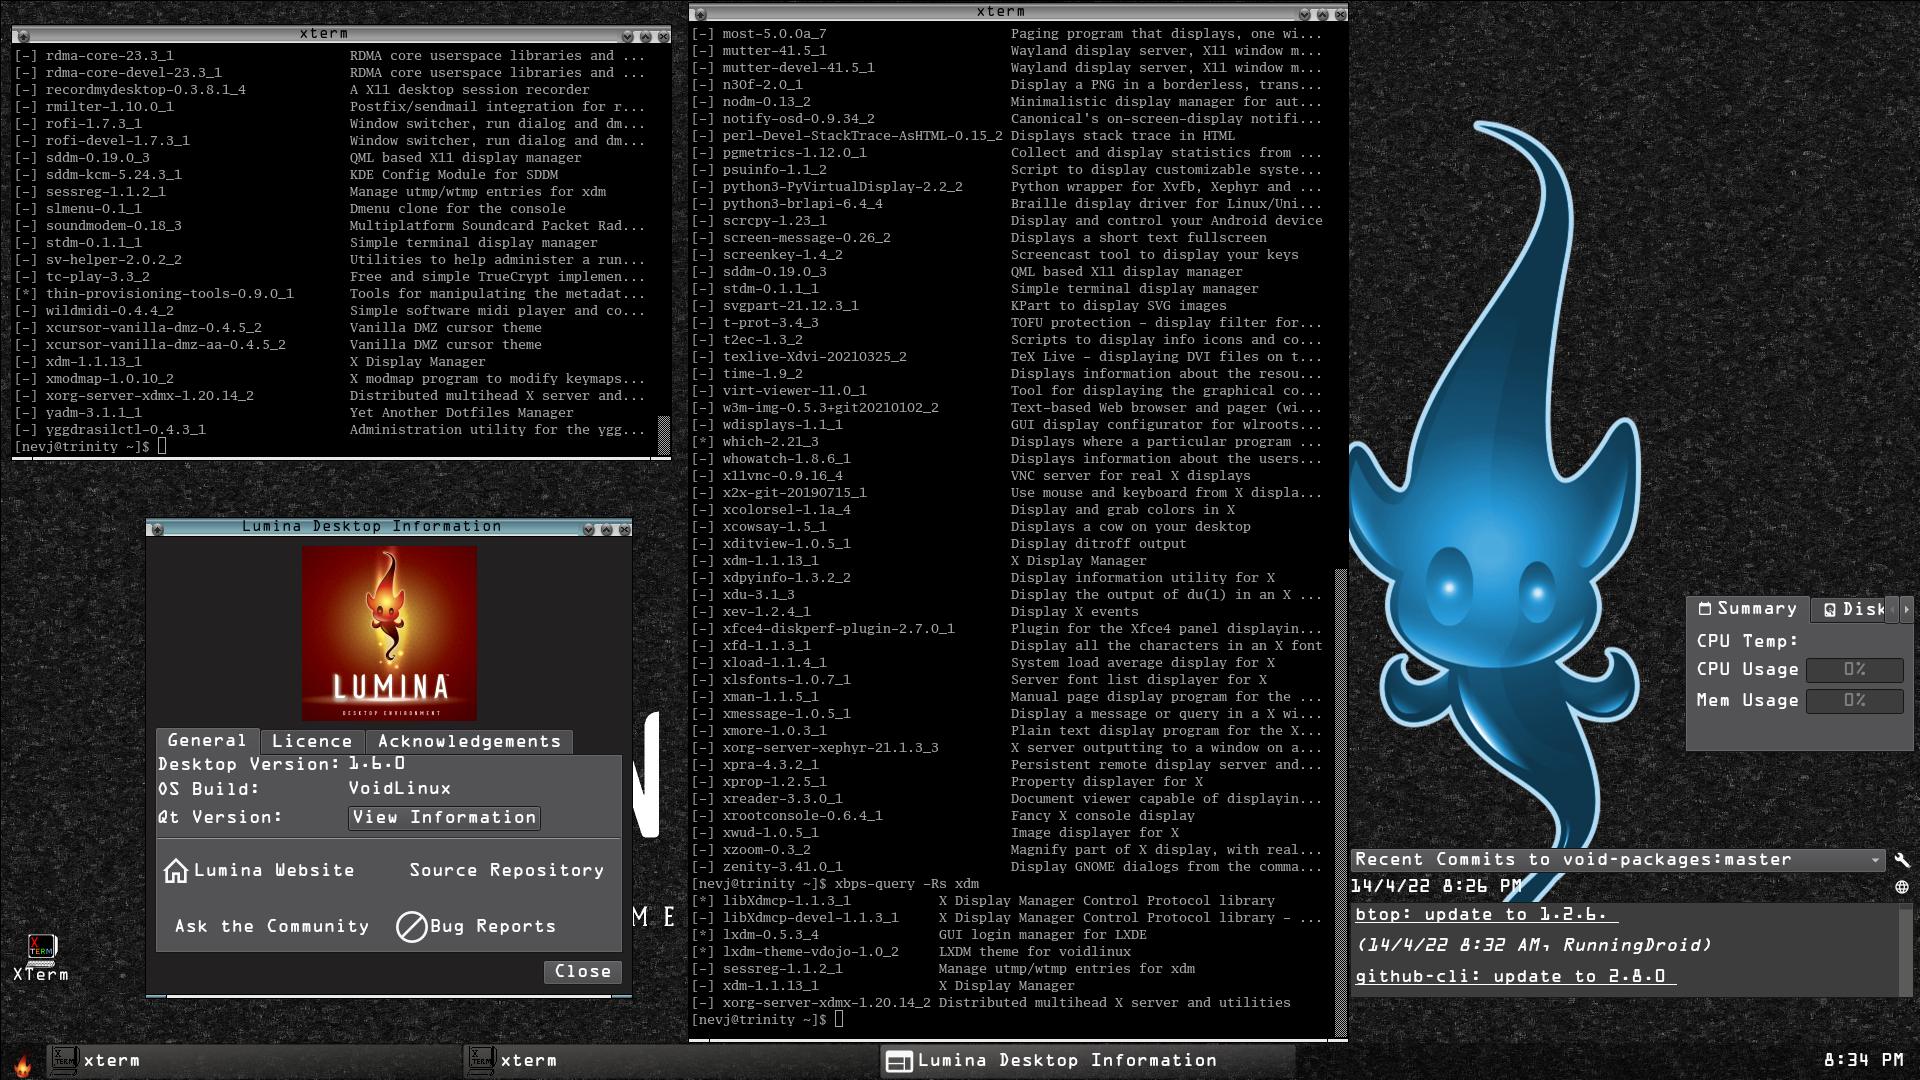
\includegraphics[totalheight=3.1in,width=1.0\textwidth]{xterm.png}
  \caption{Screenshot showing two XTerm windows, one of which has been resized vertically. Also shown is the Lumina About window.}
  \label{fig:xterm}
\end{figure}

%\end{document}


One XTerm has been resized. Xterm in Lumina has two sorts of  resizing capabilbity 
\begin{itemize}
\item  use left middle or right click on the $\wedge$ button in the top panel to resize to fullscreen, max vertical, or max horizontal, respectively.
\item drag the bottom left or right corner of the window for continuous variation of window size
\end{itemize}
 This screenshot also shows the Lumina About screen.


\clearpage

\subsection{Add a Display Manager}
Some people prefer a graphic login screen and an automatic startup of the desktop environment, a few old fashioned types persist with an alphanumeric terminal login and starting the window system by hand, as we have been doing up until now. It is either one or the other. You cant have an option.

Let us see what Display Managers are available
\begin{verbatim}
$ xbps-query -Rs display
........
[-] gdm-41.3_1                        GNOME Display Manager
[-] lightdm-1.30.0_3                  Light Display Manager
[-] sddm-0.19.0_3                     QML based X11 display manager
[-] xdm-1.1.13_1                      X Display Manager
[-] lxdm-0.5.3_4                      GUI login manager for LXDE
\end{verbatim}
We dont want {\em gdm}, that is for GNOME, and {\em sddm} is what KDE normally uses. {\em lightdm} is rather large (10Mb). That leaves the original X11 {\em xdm} or {\em lxdm} which is what {\em Xfce} uses. {\em lxdm} I know from experience with {\em Xfce} so we go with that.
\begin{verbatim}
# xbps-install lxdm
\end{verbatim}
We now have the package installed, but we need to check if the daemon is running 
\begin{verbatim}
# sv status lxdm
fail: lxdm: unable to change to service directory: file does not exist

# ls /etc/sv/lxdm
run  supervise
\end{verbatim}
So the {\em lxdm} package has put an {\em lxdm} entry in {\em /etc/sv} but it has not enabled the daemon because there is no link in {\em /var/service}. That is normal behaviour for Void, installations with {\em xbps-install} do not start a daemon if the package needs one.   So we make the link --- that will enable the service, ie the daemon will start.
\begin{verbatim}
# ln -s /etc/sv/lxdm /var/service
\end{verbatim}
Now , reboot, and the lxdm login screen comes up. Try to login, type the password, and nothing happens. Try to login as root, the same.  Something is wrong, I cant login. Failure.

Recovery mode. Go to another linux, mount the Void/Lumina root filesystem, go to {\em /etc/sv}, and disable {\em lxdm} by renaming the lxdm directory. Come out  and boot Void/Lumina and get the terminal login again. Login as root and check the {\em /etc/sv} directory. There is no login daemon .... I need to install elogind as well as the display manager. So
{\begin{verbatim}
# xbps-install elogind
\end{verbatim}
Then I need to enable elogind
\begin{verbatim}
ln -s /etc/sv/elogind /var/service
\end{verbatim}
And I need to put {\em /etc/sv/lxdm} back to its correct name.

Then reboot , and the login screen comes up again, and this time I can login. Success.

One would have thought the display manager package would drag in a login daemon, but no. And you have to start daemons by hand as well. So Void's xbps package system is not like Debian's {\em apt}, it puts software into Void, but it does not enable daemons.

The Lxdm screen offers a choice of {\em Fluxbox} or {\em Lumina} desktop environments. It also offers a choice of keyboards but only one was configured so it is a choice of one.  It also offers a shutdown button, but there is no way to come out of the screen to the terminal login prompt. That is one thing that is annoying about all Display Managers, they trap you in the graphical screen.



\subsection{The Insight File Manager}
On the command line, Insight is called {\em lumina-fm} and it has a man page. 
Insight File Manager, on its own,   has limited capability. It will only display filesystems mounted to the current system. It will not scan for other unmounted partitions or disks, in the manner of  Thunar or Dolphin . 

The {\em External Devices} tab in Insighr File Manager says "Scan for Devices" when clicked, but it shows none. I eventually discovered that it needs a helper daemon {\em ldm} called Lightweight Device Munter. So
\begin{verbatim}
xbps-install ldm
ln -s /etc/sv/ldm /var/service/ldm
\end{verbatim}
and magically the External Devices tab in Insight now shows a list of all hard disk partitions and any connected USB drives. A {\em df} shown that it mounts all devices to subdirectories in /mnt, even if not accessed. So that is different, Thunar and Dolphin only mount devices if accessed. For example
\begin{verbatim}
[nevj@trinity ~]$ df
Filesystem      1K-blocks     Used Available Use% Mounted on
devtmpfs         32879776        0  32879776   0% /dev
tmpfs            32918284        0  32918284   0% /dev/shm
tmpfs            32918284     1284  32917000   1% /run
/dev/sda1       190923068  6666832 174485128   4% /
cgroup           32918284        0  32918284   0% /sys/fs/cgroup
tmpfs            32918284       12  32918272   1% /tmp
/dev/sda4      1116282132 62838976 996716220   6% /mnt/Common
/dev/sda6          201633      124    201510   1% /mnt/EFI_SYSTEM
/dev/sda7       310467116 27865776 266760780  10% /mnt/rootVoid
/dev/sdb1       100658948 20389360  75133292  22% /mnt/LinuxRoot1
/dev/sdb10      201454560  1028396 190169780   1% /mnt/LinuxHome4
/dev/sdb11        1021984     3484   1018500   1% /mnt/274A-6A33
/dev/sdb12      201454560  7448768 183749408   4% /mnt/Linuxroothome
/dev/sdb3       201451180 18806952 172388016  10% /mnt/LinuxHome1
/dev/sdb5       100660656 17956896  77567376  19% /mnt/LinuxRoot2
/dev/sdb6       201454560  7398156 183800020   4% /mnt/LinuxHome2
/dev/sdb7       100267080 13375812  81754884  15% /mnt/LinuxRoot3
/dev/sdb8       201454560 11092296 180105880   6% /mnt/LinuxHome3
/dev/sdb9       100660656 11591172  83933100  13% /mnt/LinuxRoot4
\end{verbatim}
Everything is mounted!  That might annoy some, but it actually suits me. I do a lot of mounts looking at other systems.

 Insight's display of files and folders in more than adequate. It has thumbnails in an unusual arrangement alongside the filenames.

I thought it was worth having a look at other possible choices of File Manager. Within those built on Qt there are PCManFM, Qtfm, and Dolphin. I tried PCManFM and it offered nothing over Insight. Dolphin, of course , is well known , but it comes with a huge KDE baggage. So I settled for Qtfm, which according to the man pages deals with automounts of USB removable devices via a daemon called {\em qtfm-tray}. I could not get Qtfm to mount a removable USB drive, but I kept it as an alternative to Insight with a more conventional thumbnail display of files and folders.  In my opinion Insight is a better File Manager than Qtfm.

Figure ~\ref{fig:fm} shows screenshots of the Insight and Qtfm file managers
%\documentclass{article}
%\usepackage{graphicx,subfigure}
%\usepackage{caption,rotating}
%\begin{document}

\begin{figure}[p]
\centering
 \subfigure[Insight File Manager]{
    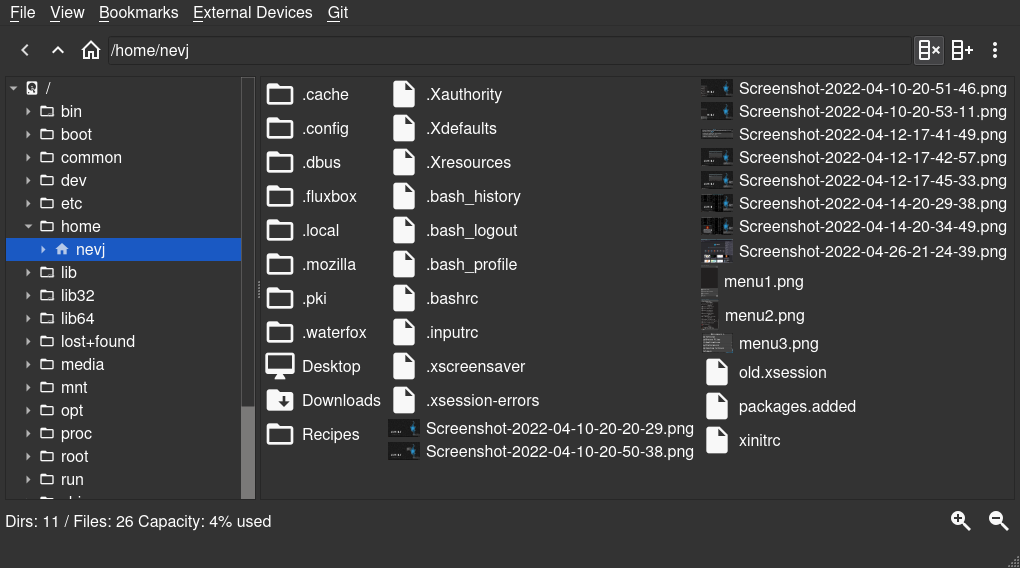
\includegraphics[scale=0.60]{insight.png}
  }
 \subfigure[QtFM File Manager]{
    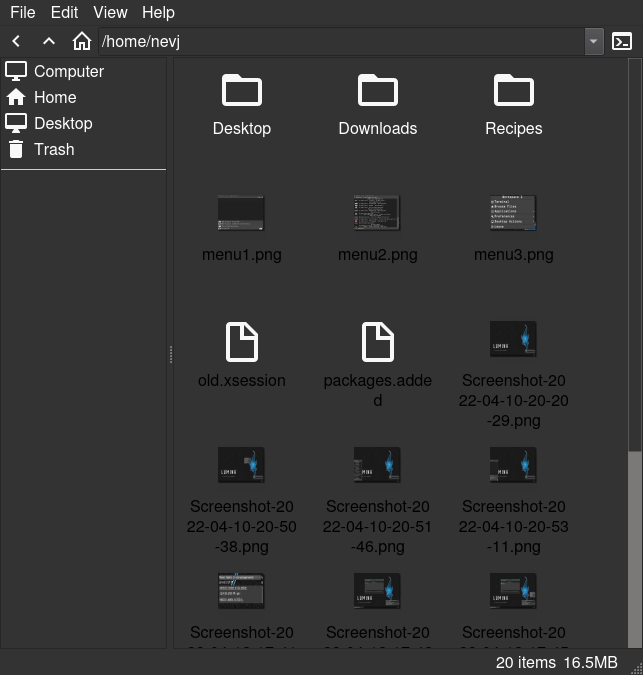
\includegraphics[scale=0.60]{qtfm.png}
  }
  \caption{Screenshots of the Lumina Insight File Manager and the QtFM File Manager}
\vfill
  \label{fig:fm}
\end{figure}

%\end{document}


These are two lightweight options. If they are not adequate, the best choice is Dolphin.  Using a non-Qt file manager is possible, but it leads to downloads of another whole support framework, just to run the file manager.

\subsection{Other applications packaged with Lumina}
The list of applications that come with Lumina is as follows
\begin{verbatim}
 man -k lumina
lumina-archiver(1) - a graphical front-end to tar. Manages and
 creates archives.
lumina-calculator(1) - full scientific calculator with a simple
 interface.
lumina-config(1) - modifies different desktop settings.
lumina-desktop(1) - Binary used to run or communicate with the
 desktop.
lumina-fileinfo(1) - views properties of files. Includes creator
 for XDG application registrations and XDG-compliant desktop entries.
lumina-fm(1) - is a utility used for browsing and interacting with
 files on the system.
lumina-info(1) - view information about the current desktop.
lumina-mediaplayer(1) - a graphical utility to play media files and
 stream online radio services.
lumina-open(1) - a graphical front-end to xdg-open. Opens files or
 links with the proper application.
lumina-photo(1) - a graphical utility to open pictures.
lumina-screenshot(1) - a utility to take and save screenshots of
 the desktop.
lumina-search(1) - searches for files and applications.
lumina-textedit(1) - plaintext editor.
lumina-xconfig(1) - graphical front-end to xrandr, which manages
 monitor configurations.
start-lumina-desktop(1, 8) - Basic binary that starts a new Lumina
 session for the current user.
\end{verbatim}
There is no browser or terminal; we have dealt with adding Xterm - we add abrowser in the next section.
 
The Lumina PDF Viewer ( called lumina-pdf, but it has no man page so did not appear in above list) is OK at higher magnifications, but at default setting text is a bit dotty. It has no page thumbnails. It is definately inferior to {\em evince} or {\em okular} for displaying \LaTeX \hspace{.1cm} generated PDF files. 

The Lumina Media Player (lumina-mediaplayer) has a man page , but does not function. It will not even open a file. One would need to replace it with a reliable functioning player like {\em VLC}.


The Lumina Calculator works, and as a nice scientific function key. 

The Lumina Archiver is a graphical front end to {\em tar}. It also seems to have a USB 'burn' (ie write) option.

The Lumina File Information (lumina-fileinfo) app does a mix of the information obtained with {\em ls -l}  and {\em file}. It has a man page.

The Lumina Image Viewer (lumina-photo) works. It can zoom and that is about all. The back and forward arrows do not work if it opens a single image so it can not skip over the images in a directory.

The Lumina Screenshot app (lumina-screenshot) is excellent. All the Figures in this document were made with it. 

Lumina Search is something unique. It will search for either files or applications. For example if I set it to search applications and tyoe 'browse', it finds the Waterfox Web Browser, which was installed outside the Void package system. If I set it to search files or directories and type 'Desktop', it finds {\em ~/Desktop} directory and lists its contents. It has a man page. For a files search, one can exclude directories. It also has a launcher, and the launch works.

The Lumina Text Editor (lumina-textedit) is like {\em nano}. It has a man page. In the background menu, it is callled 'Terminal' which is confusing.

There are a number of other Lumina apps which are for configuration - Desktop Configuration, Monitor Configuration (also called Screem Configuration), Theme Engine ( also called Theme Settings), Manage Printing, and Lumina Desktop Information.

Most Lumina apps work, but offer a very basic functionality. There is some annoying inconsistency in naming.

\subsection{Add a web browser}
The lumina desktop prompts for {\em firefox} as the default browser, but it is not installed.  Let us see what browsers are available in Void repository
\begin{verbatim}
xbps-query -Rs browser
.....
[-] dillo-3.0.5_13                                Small and light graphical ..
[-] eolie-0.9.62_4                                Web browser for GNOME
[-] epiphany-41.3_1                               Intuitive GNOME web browser
[-] falkon-3.2.0_1                                Cross-platform Qt Web Browser
[-] firefox-98.0_1                                Mozilla Firefox web browser
[-] firefox-esr-91.6.0_1                          Mozilla Firefox web browse...
[-] konqueror-21.12.3_1                           KDE File Manager & Web Bro...
[-] kristall-0.3_2                                Small-Internet Browser
[-] midori-9.0_1                                  Lightweight web browser us...
[-] netsurf-3.10_3                                Free, open source web brow...
[-] otter-browser-1.0.02_1                        Web browser aiming to recr...
[-] surf-2.1_1                                    Simple web browser based o...
[-] vimb-3.6.0_1                                  Fast and lightweight web b...
[-] opera-84.0.4316.31_1                          Fast, secure, easy to use ...
[-] nyxt-2.2.4_3       Keyboard-oriented, extensible web-browser
\end{verbatim}
I have omitted text based browsers. Quite a selection but no Brave, Chrome, Vivaldi, or Librewolf. Epiphany, Eolie, Falkon, Konqueror are Gnome or KDE specific. Vimb, Surf, are minimalist keyboard driven. That leaves Firefox, Opera, Midori, Netsurf, Nyxt and Dillo. 

Lets have a look at the download sizes -- we have firefox (65Mb), opera (92Mb), nyxt (23Mb), netsurf (1912Kb), dillo (1255Kb), midori (845 Kb). First let us try a mid-range choice - nyxt.
\begin{verbatim}
xbps-install nyxt
\end{verbatim}
Nyxt comes up with a reasonable looking window, but the interface is not user friendly. It asks for things I dont understand and no button I press seems to get me to the point where I can enter a web address and do some browsing. I am probably a bit brutal, but that rules nyxt out. 
\begin{verbatim}
xbps-remove nyxt
\end{verbatim}

The tiny browsers, Dillo, Netsurf, and Midori; I look at each in turn, and they are all functional, but very elementary. 

So for the moment I install firefox
\begin{verbatim}
xbps-install firefox-esr
\end{verbatim}
And that works, just the same as in any other Linux

I am not happy with any of the Void browser offerings, so I decide to look, outside the Void repository, at two semi-independent firefox clones... LibreWolf and Waterfox.

LibreWolf has a Gitlab site~\cite{libr:22} from which one can download source code either as a tarball or by  cloning the Git repository.  They do not have a build for Void Linux.  I chose the clone method. I followed the build instructions, but there were unrtesolved difficulties with compiling. The attempt to get LibreWolf  into Void was abandoned.

Waterfox has a website(~\cite{wate:22} which offers downloads of packaged binaries for linux-x86,linux-ARM, Windows, MacOS. The download for Linux is a .tar.bz2 file. You unpack the bz2 file, untar it, and simply copy the Waterfox binary and some libraries to wherever you want to install them. I used /usr/local/bin and /usr/local/lib. Full details of downloading and installing Waterfox are given in a separate document~\cite{waterfox:22}

Figure~\ref{fig:waterfox}  shows the window of my Waterfox browser running in the Lumina desktop in Void Linux. 
%\documentclass{article}
%\usepackage{graphicx,subfigure}
%\begin{document}

\begin{figure}[!h]
  \centering
   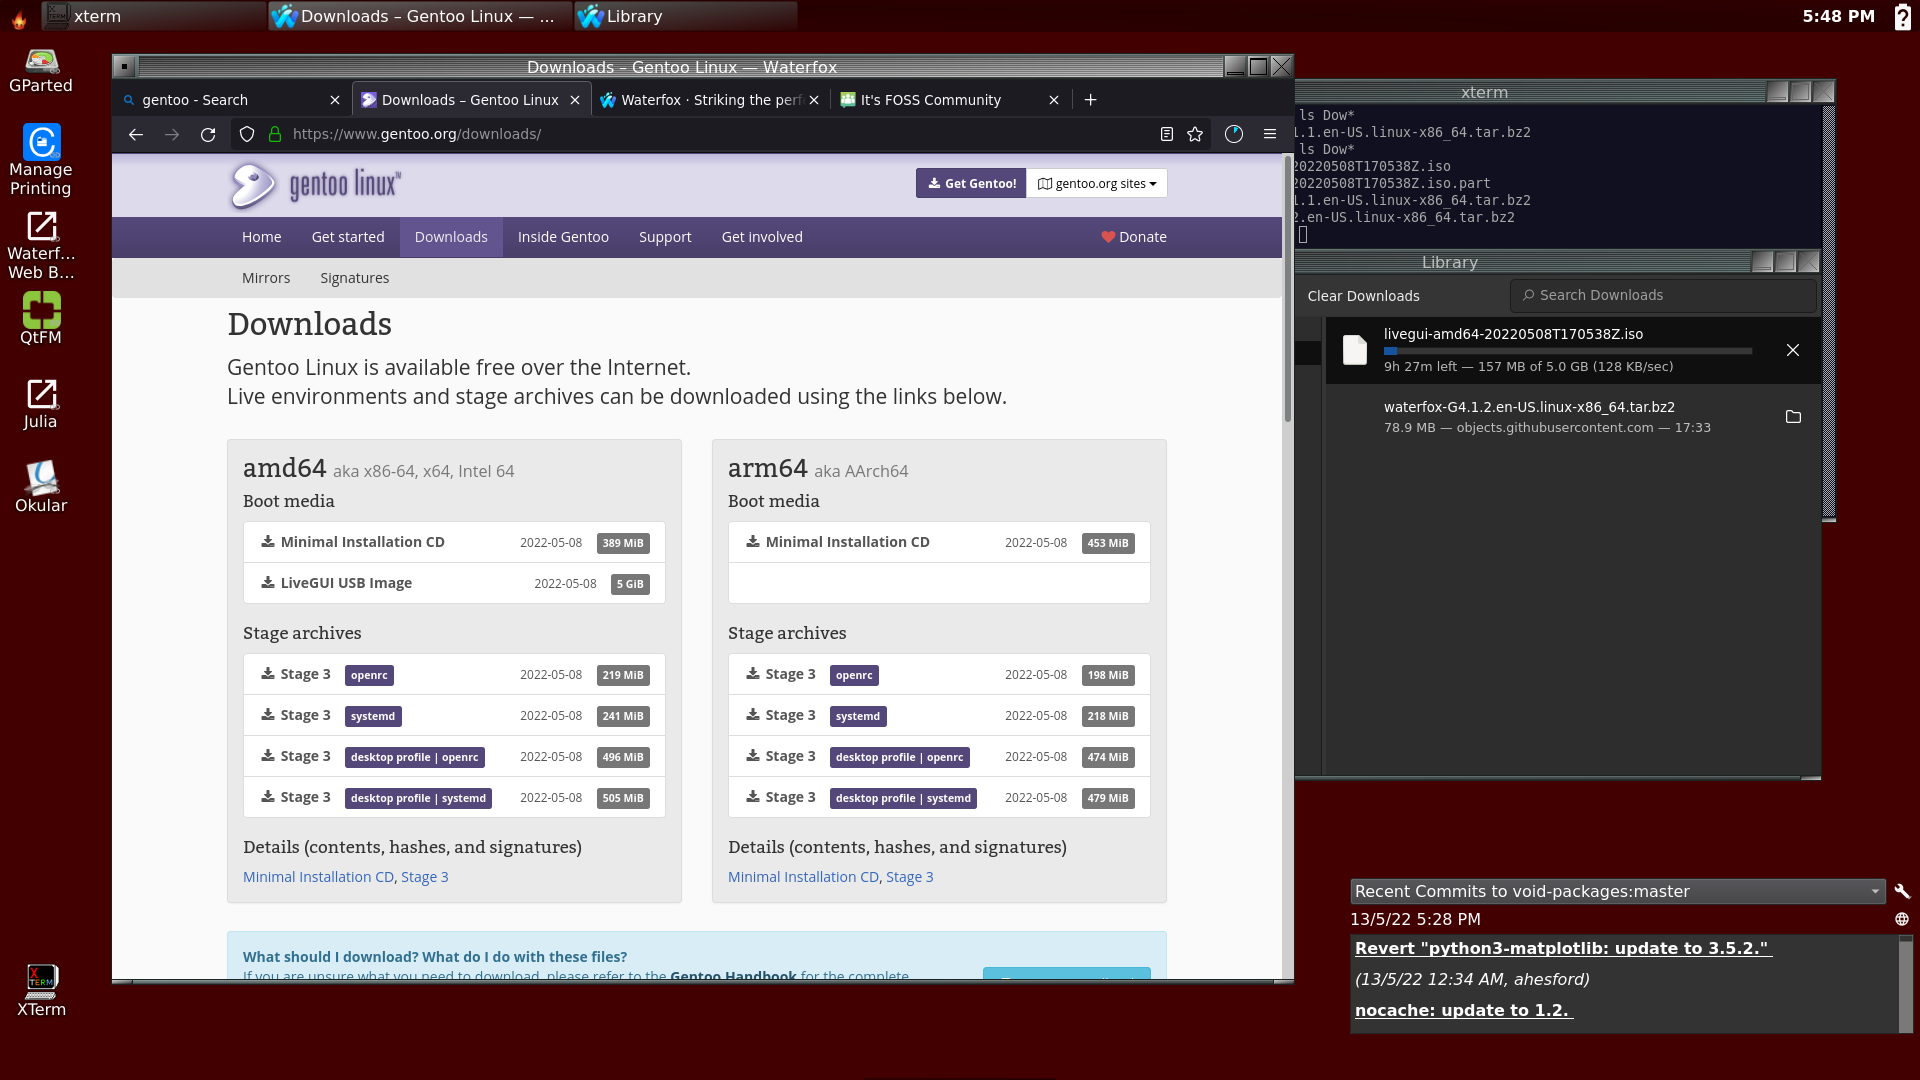
\includegraphics[totalheight=3.2in,width=1.0\textwidth]{watlum.png}
  \caption{Screenshot of Waterfox browser window running in Lumina Desktop}
  \label{fig:waterfox}
\end{figure}

%\end{document}


It looks just like Firefox.

\section{Configuration and plugins}
What has been  shown so far is just the default desktop layout.
Lumina is highly configurable. It uses plugins to allow the user to alter the desktop layout. There is a full description of plugins on a Github site~\cite{plug:22} This site describes every plugin and how to use it to customize the desktop.

It has been shown that the plugin concept is so flexible that you can transform the Lunina Desktop into an almost perfect emulation of an Xfce, Gnome/Mate or Windows desktop. Figure~\ref{fig:win} shows an example of Lumina set up to emulate the Windows layout
%\documentclass{article}
%\usepackage{graphicx,subfigure}
%\begin{document}

\begin{figure}[!h]
  \centering
   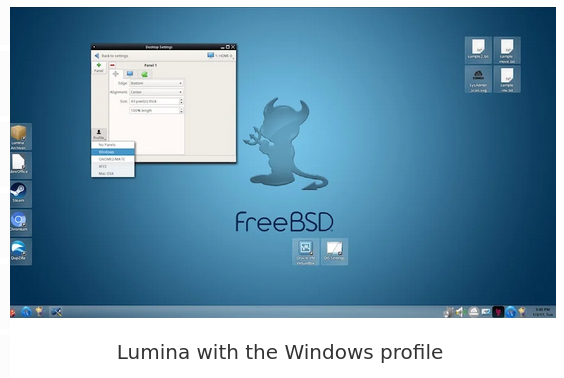
\includegraphics[totalheight=3.5in,width=1.0\textwidth]{luminawin.png}
  \caption{Screenshot of Lumina Desktop emulating the Windows desktop layout - picture courtesy of the Fossbytes website}
  \label{fig:win}
\end{figure}

%\end{document}


This figure came from the fossbytes site~\cite{tran:22}, which you should visit to see other other examples emulating Gnome/Mate and Xfce.

We might try some layout and presentation variations, just to see it working.  I spent about 10 minutes just altering the panel settings and the background, and came up with Figure~\ref{fig:oz}
%\documentclass{article}
%\usepackage{graphicx,subfigure}
%\begin{document}

\begin{figure}[!h]
  \centering
   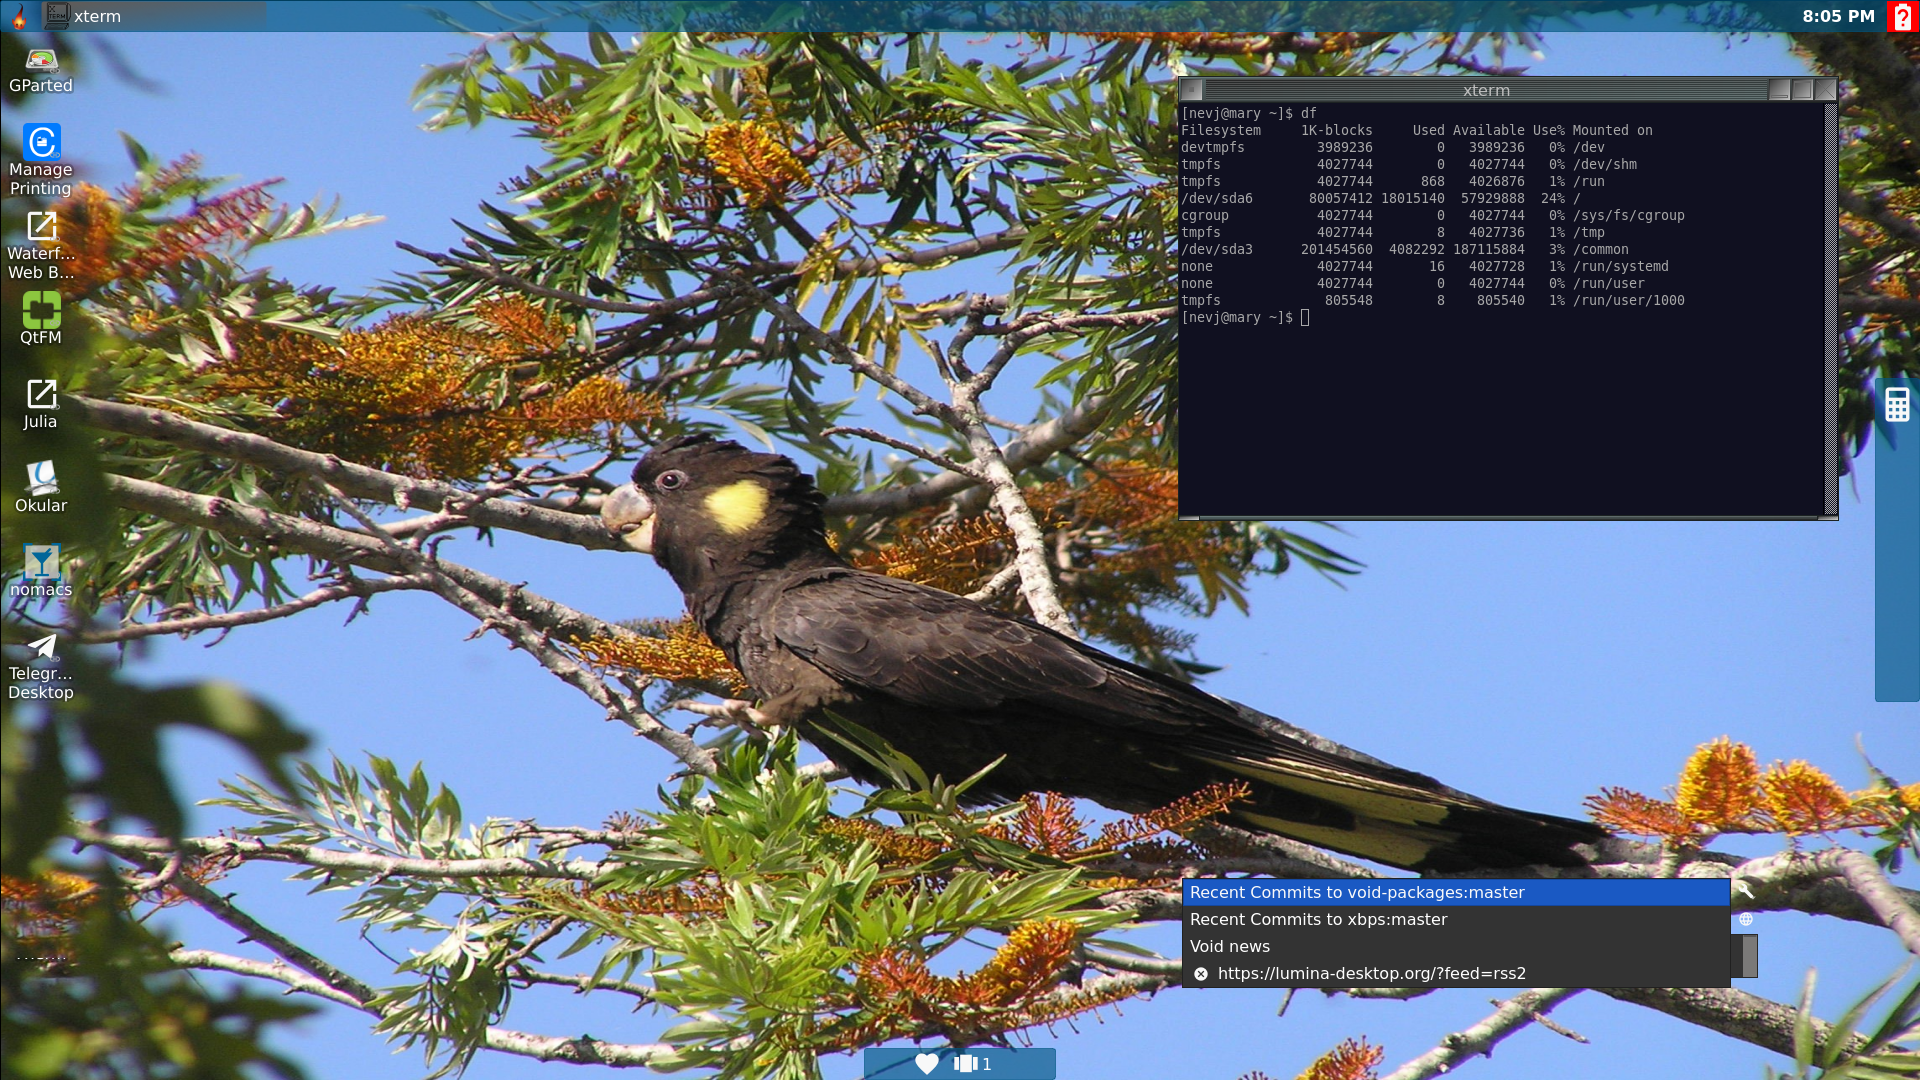
\includegraphics[totalheight=3.2in,width=1.0\textwidth]{luminaoz.png}
  \caption{Screenshot of Lumina Desktop configured to emulate Xfce panel layout and with an Australian backdrop}
  \label{fig:oz}
\end{figure}

%\end{document}


I did not edit any configuration files, it is all done with Desktop Settings GUI. See the Github Plugin site~\cite{plug:22} for details.
You can see the system tray at the top of screen, the panel with favourites and workspaces at the bottom centre, and an extra panel at the right side with a calculator icon. The right side panel is a popup. The icon for the Applications Menu is at the top left corner.There are some application icons on the background in addition to the RSS Feed embedded plasmid. The background is a uniquely Australian shot of a Black Cockatoo on a Silky Oak tree. 

One would normally use such a bright desktop in a well lit area during the day. As I do most of my computing at night, I prefer a more dull desktop with a bias towardd the red end of the spectrum. You will see some examples of that in the next section.

The point of all this fiddling with configurations is to show that Lumina is very adaptble. You can make it look like any of the usual desktops or make your own unique design. It is easily changed; you can swap desktops with a few clicks.


\clearpage
\section{Add my normal application software}
The things I use most are R, and \LaTeX \hspace{.1cm} and a PDF viewer. I am not a big consumer of GUI apps other than a browser and command line terminals. R uses graphic windows. 
Installing R, and \LaTeX \hspace{.1cm} in Void is quite straightforward
\begin{verbatim}
xbps-install R-4.1.3_1
xbps-install texlive-basic
xbps-install texlive-fonts-extra
xbps-install gcc-fortran
xbps-install okular
\end{verbatim}
That is a mass of downloads, but simple to do. 

Now what I need to do is carry out some normal work with R and \LaTeX \hspace{.1cm} and see if {\em lumina} supports everything. Firstly R; I have to add a collection of R packages to the R installation. We will omit the details of that; R is a world of its own. Figure~\ref{fig:rgraph} shows an xterm running R and an X11 window with R graphics. 
%\documentclass{article}
%\usepackage{graphicx,subfigure}
%\begin{document}

\begin{figure}[!h]
  \centering
   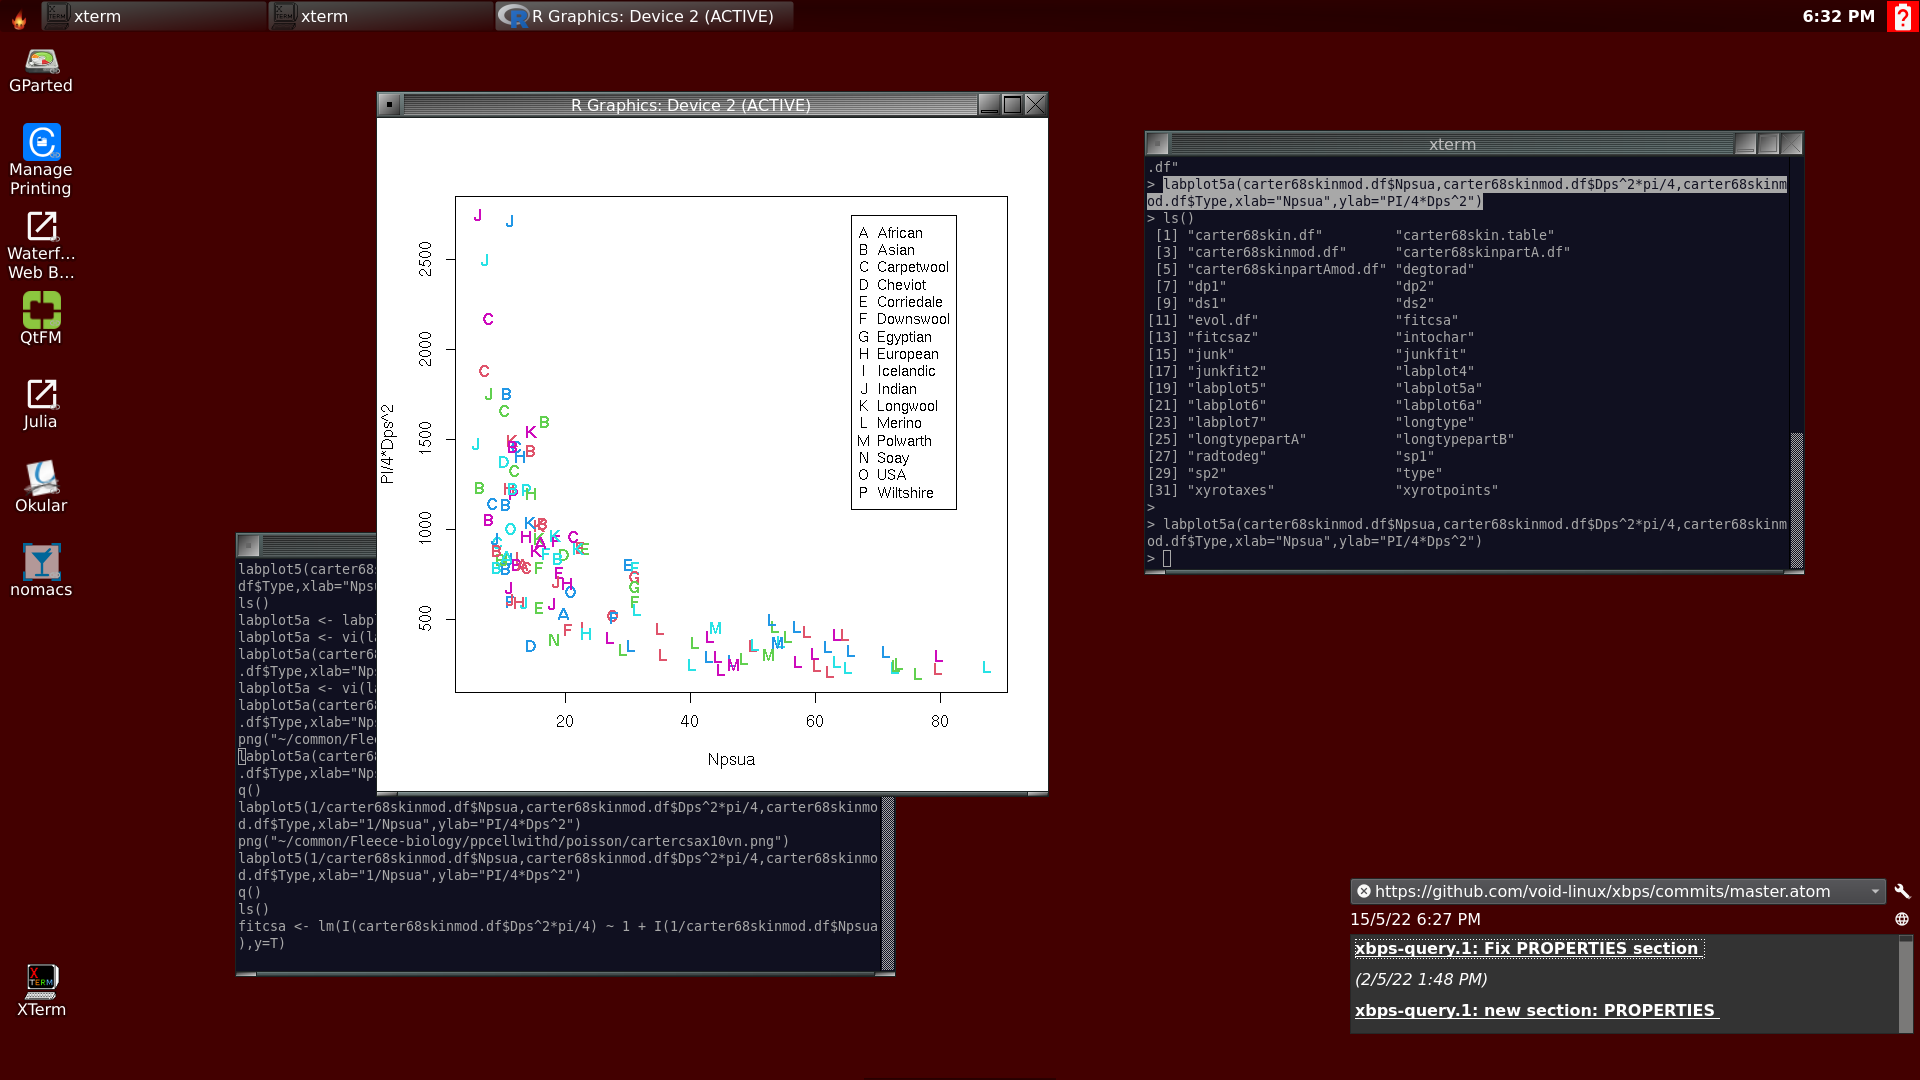
\includegraphics[totalheight=3in,width=1.0\textwidth]{rgraph.png}
  \caption{Screenshot of Lumina Desktop with R running in an Xterm and a graph drawn by R in an X11 window}
  \label{fig:rgraph}
\end{figure}

%\end{document}


Everything works, all the fonts are present, X11 graphics support is there. As far as an R user is concerned, it is just like working in any other DTE.

Now lets try out \LaTeX. Figure~\ref{fig:latex} shows an Xterm editing a .tex file and the resulting .pdf file being rendered dynamically by okular in a separate window.
%\documentclass{article}
%\usepackage{graphicx,subfigure}
%\begin{document}

\begin{figure}[!h]
  \centering
   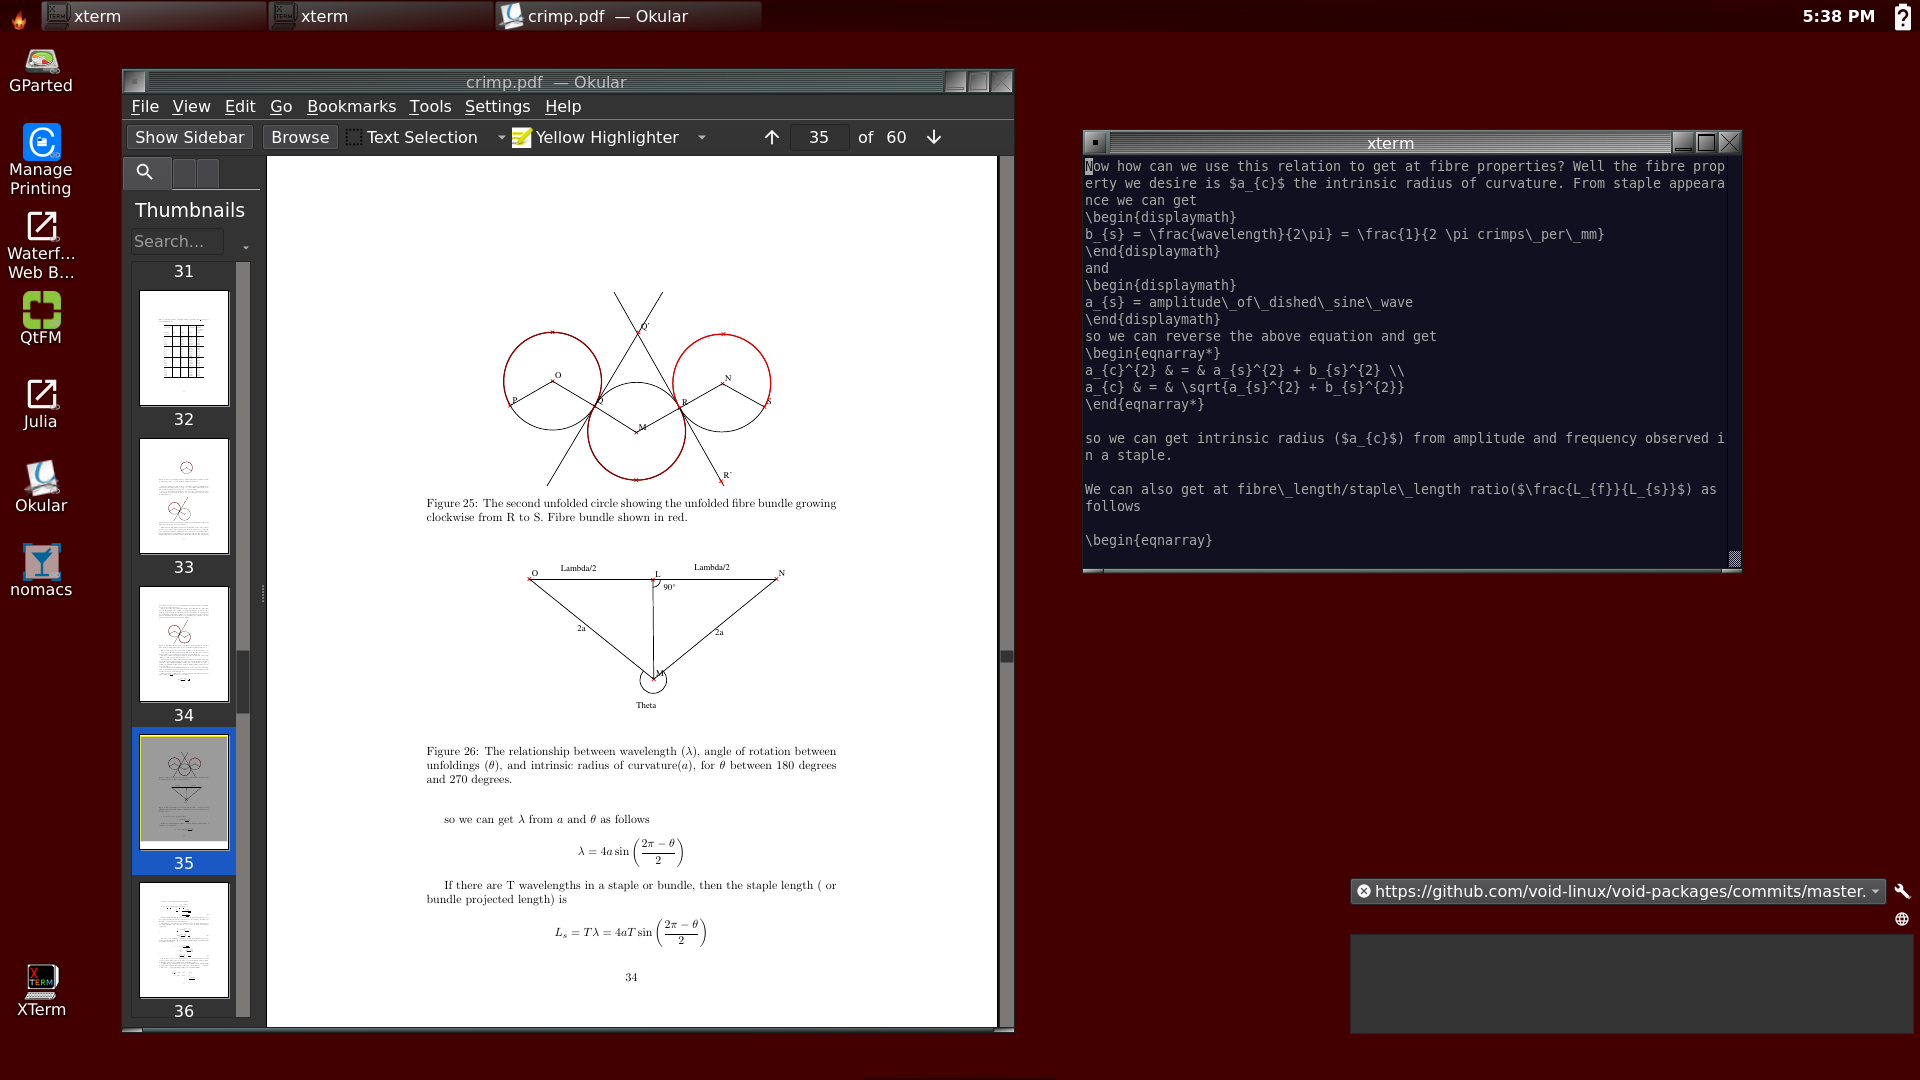
\includegraphics[totalheight=3in,width=1.0\textwidth]{latex.png}
  \caption{Screenshot of Lumina Desktop with vi running in an Xterm editing a .tex file and a rendering of the resulting .pdf file  by okular in  an X11 window}
  \label{fig:latex}
\end{figure}

%\end{document}


Again everything works. I chose okular (rather than evince or atril) because it is Qt based. The native Lumina PDF Viewer is inadequate for my purpose. When I translate the .tex file to a .pdf file, the okular window updates dymnamically. The rendering of equations and drawings is perfect. 

\section{Pros and cons for Lumina}
It is not all black and white, there are neutral considerations too.
\subsection{Pros}
\begin{itemize}
\item multi-platform support - runs on BSD, Linux, Macos
\item configurable - can make it loook like any other DTE or something unique
\item modern features - has app embedding like KDE plasma
\end{itemize}

\subsection{Cons}
\begin{itemize}
\item incomplete - two of the inbuilt Lumina apps do not work well enough to be useful. One can substitute better apps.
\item not 'out of the box' - requires some install and setup effort and you will end up adding a number of personal choices of apps.
\item long term development uncertain - it is maintained at the moment
\end{itemize}

\subsection{Neutral issues}
\begin{itemize}
\item unfamiliar - has a BSD background 
\item 'light' desktop - comes with a small number of inbuilt apps. You have to add your favourite apps.
\item  Qt based - that is modern.
\end{itemize}

\section{Discussion}
The bottom line is ... would anyone use Lumina as their daily work environment? This investigation has shown that there is no reason to shun it. I am going to continue working in it for a while and just see where it leads.

The biggest issue longterm is support. There is development at the moment, and the Lumina website~\cite{lumi:22} is calling for contributors.  Its future depends on continuing development.


\begin{thebibliography}{99}

\bibitem{foss:21}
FOSS article on Project Trident
URL https://news.itsfoss.com/project-trident-discontinues/

\bibitem{libr:22}
LibreWolf source code website.
URL https://gitlab.com/librewolf-community/browser/source

\bibitem{lumi:22}
Lumina Desktop site
URL https://lumina-desktop.org

\bibitem{plug:22}
Plugin Github site
URL https://github.com/lumina-desktop/lumina-docs/blob/master/luminaplugins.rst

\bibitem{tran:22}
Transforem your OS into a Mate, Xfce, Windows, aor OSX UI with Lumina 1.2 Desktop.
URL https://fossbytes.com/lumina-1-2-desktop-download-features/

\bibitem{wate:22} 
Waterfox website. URL https://www.waterfox.net

\bibitem{waterfox:22}
Install the Waterfox browser on a Linux system. Neville Jackson. URL https://githyb.com/nevillejackson/Unix/tree/main/waterfox/waterfox.pdf


\end{thebibliography}
\end{document}
